% !TeX root = molecular-dynamics.tex
% !TeX outputDirectory = ../../tutorial-pdfs/

\documentclass[english,course]{lecture}
\usepackage{amsmath}
\usepackage{hyperref}
\usepackage{tikz}
\usetikzlibrary{shapes.geometric, arrows, positioning}

% Document metadata
% \ccode{WCGMS BCMB}
\title{Knowledge Base}
\subtitle{Molecular Dynamics}
\shorttitle{Inspired by Jay Ponder}
\subject{Biophysics}
\author{Sukrit Singh}
\email{sukrit.singh@choderalab.org}
% \date{02}{08}{2024}
% \dateend{09}{08}{2024}
\attn{Introduction to dynamical systems and molecular simulations}
\morelink{http://choderalab.org}
%
% Begin document
\begin{document}

\vfill
\eject

%%%%%%%%%%%%%%%%%%%%%%%%%%%%%%%%%%%%%%%%%%%%%%%%%%%%%%%%%%%%%%%%%%%%%%%%%%%%%%%%%%%%%%%%%%%%%%%%%%%%%%%%%%%%%%%%%%%%%%%%%%%%%%%%%%%%
%% COURSE MATERIALS
%%%%%%%%%%%%%%%%%%%%%%%%%%%%%%%%%%%%%%%%%%%%%%%%%%%%%%%%%%%%%%%%%%%%%%%%%%%%%%%%%%%%%%%%%%%%%%%%%%%%%%%%%%%%%%%%%%%%%%%%%%%%%%%%%%%%

\section{Recommended reading and supportive texts}

\subsection*{Recommended reading}

\noindent {\bf Molecular Driving Forces}, Dill and Bromberg\\
Chapter 15 ("Binding Models and Binding Sites") \href{https://tinyurl.com/dill-bromberg-preview}{[PDF (click "Preview this Book")]}\\

% \noindent {\bf Understanding Molecular Simulation: From Algorithms to Applications}, Frenkel and Smit \\
% A detailed resource on the principles and techniques of molecular simulation.
% \href{https://www.amazon.com/Understanding-Molecular-Simulation-Algorithms-Applications/dp/0122673514}{[Amazon]}

\vfill
\eject

%%%%%%%%%%%%%%%%%%%%%%%%%%%%%%%%%%%%%%%%%%%%%%%%%%%%%%%%%%%%%%%%%%%%%%%%%%%%%%%%%%%%%%%%%%%%%%%%%%%%%%%%%%%%%%%%%%%%%%%%%%%%%%%%%%%%
%% MOLECULAR DYNAMICS BASICS
%%%%%%%%%%%%%%%%%%%%%%%%%%%%%%%%%%%%%%%%%%%%%%%%%%%%%%%%%%%%%%%%%%%%%%%%%%%%%%%%%%%%%%%%%%%%%%%%%%%%%%%%%%%%%%%%%%%%%%%%%%%%%%%%%%%%

\section{Molecular Dynamics Basics}

Molecular dynamics (MD) is a computational simulation technique used to model the physical movements of atoms and molecules over time. By using MD, researchers can study the structural dynamics of biological molecules under various conditions.

\subsection{Hamiltonian Dynamics}

Hamiltonian dynamics form the basis of classical MD simulations, where the total energy of the system is described by the Hamiltonian \(H\), which is the sum of kinetic and potential energies:

\[
H(q, p) = \sum_{i} \frac{p_i^2}{2m_i} + V(q)
\]

- \(q\) and \(p\) are the position and momentum coordinates, respectively.
- \(m_i\) is the mass of particle \(i\).
- \(V(q)\) is the potential energy as a function of positions.

Hamilton's equations of motion are:

\[
\frac{dq_i}{dt} = \frac{\partial H}{\partial p_i}, \quad \frac{dp_i}{dt} = -\frac{\partial H}{\partial q_i}
\]

These equations describe how the system evolves over time, preserving total energy in an isolated system.

\subsection{Langevin Dynamics}

Langevin dynamics introduces stochastic and damping forces to the Hamiltonian framework, allowing simulations to model systems interacting with a heat bath, which is more realistic for many biological systems:

\[
m_i \frac{d^2q_i}{dt^2} = -\frac{\partial V}{\partial q_i} - \gamma \frac{dq_i}{dt} + \eta_i(t)
\]

- \(\gamma\) is the friction coefficient.
- \(\eta_i(t)\) is a random force representing thermal fluctuations, typically modeled as Gaussian white noise.

The Langevin equation is advantageous for simulating systems at constant temperature and efficiently exploring conformational space by overcoming potential energy barriers.

\subsection{The Concept of State, System, and Integrator}

\begin{itemize}
    \item \textbf{State}: In MD simulations, a \emph{state} refers to the complete set of positions and velocities of all particles at a given time. This information is crucial for computing subsequent trajectories and thermodynamic properties.
    
    \item \textbf{System}: A \emph{system} in MD is the collection of particles being simulated, along with the interactions, constraints, and conditions applied (e.g., periodic boundary conditions, temperature control).
    
    \item \textbf{Integrator}: The \emph{integrator} is the algorithm used to solve the equations of motion, updating particle positions and velocities. Common integrators include the Verlet and Velocity-Verlet algorithms, which offer a balance between computational efficiency and accuracy.
\end{itemize}

\subsection{MD Integration Steps}

Running an MD simulation involves iteratively applying the integrator to evolve the state of the system over discrete time steps:


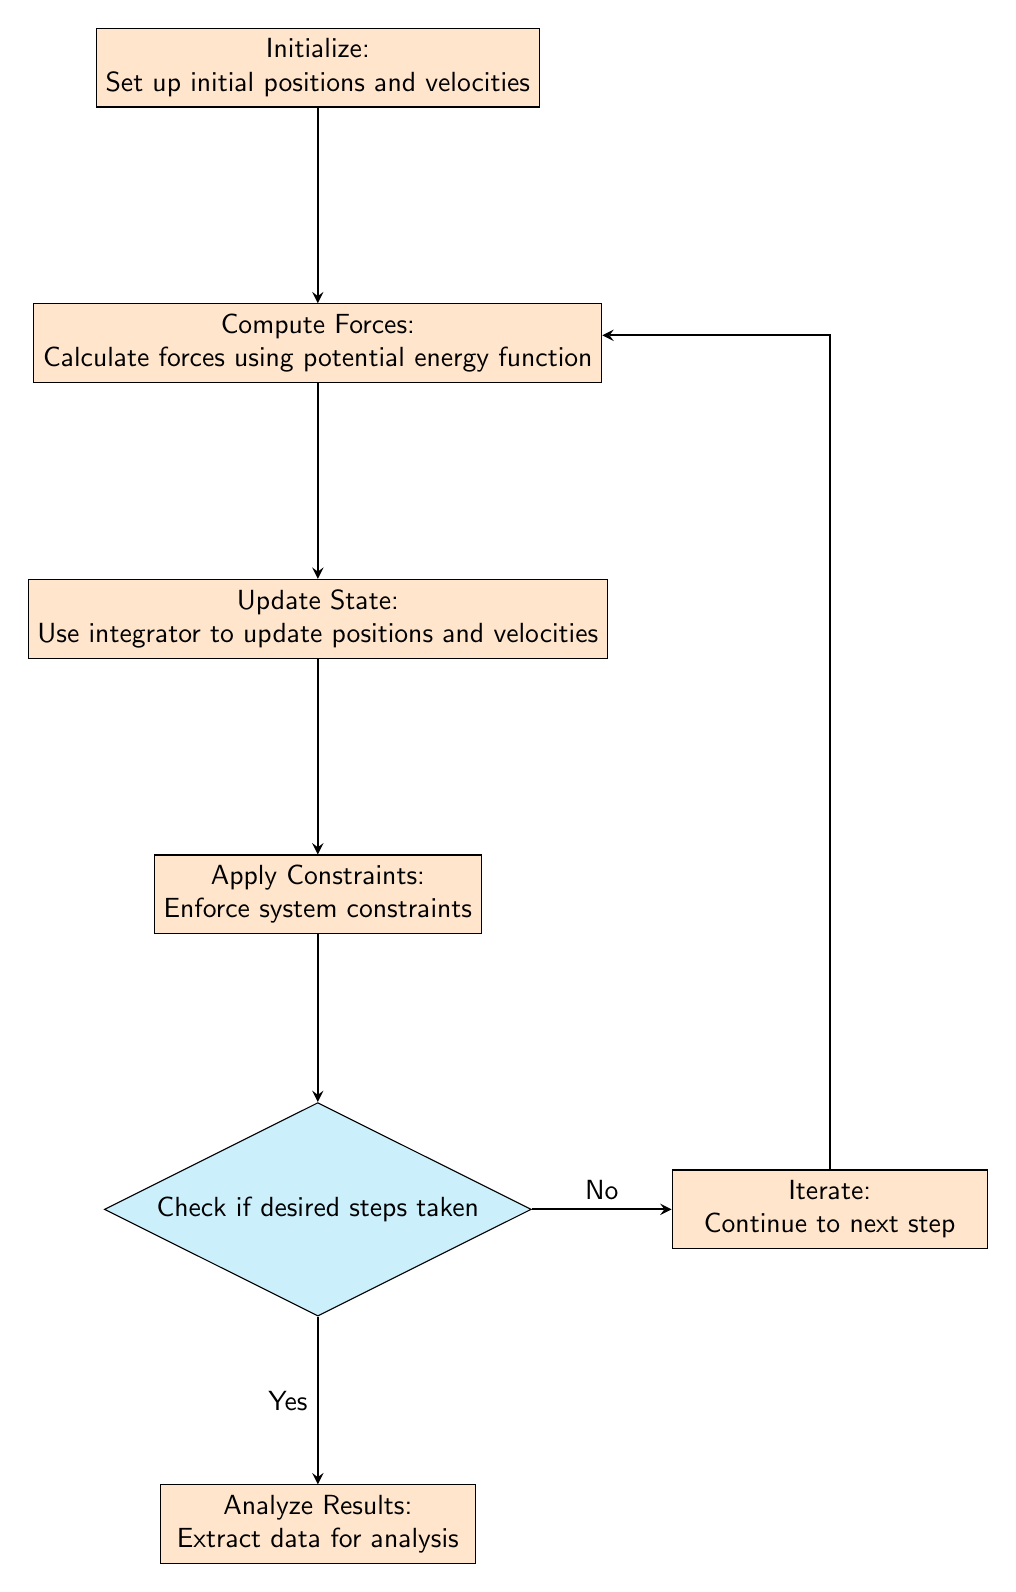
\begin{tikzpicture}[node distance=2.5cm, every node/.style={fill=white, font=\sffamily}, align=center]
    % Define styles for the blocks
    \tikzstyle{process} = [rectangle, minimum width=4cm, minimum height=1cm, text centered, draw=black, fill=orange!20]
    \tikzstyle{decision} = [diamond, aspect=2, text centered, draw=black, fill=cyan!20]
    \tikzstyle{arrow} = [thick,->,>=stealth]

    % Define nodes in the flowchart
    \node (initialize) [process] {Initialize: \\ Set up initial positions and velocities};
    \node (compute) [process, below of=initialize, yshift=-1cm] {Compute Forces: \\ Calculate forces using potential energy function};
    \node (update) [process, below of=compute, yshift=-1cm] {Update State: \\ Use integrator to update positions and velocities};
    \node (constraints) [process, below of=update, yshift=-1cm] {Apply Constraints: \\ Enforce system constraints};
    \node (check) [decision, below of=constraints, yshift=-1.5cm] {Check if desired steps taken};
    \node (iterate) [process, right of=check, xshift=4cm] {Iterate: \\ Continue to next step};
    \node (analyze) [process, below of=check, yshift=-1.5cm] {Analyze Results: \\ Extract data for analysis};

    % Draw arrows between the nodes
    \draw [arrow] (initialize) -- (compute);
    \draw [arrow] (compute) -- (update);
    \draw [arrow] (update) -- (constraints);
    \draw [arrow] (constraints) -- (check);

    % Decision arrows
    \draw [arrow] (check.east) -- node[anchor=south] {No} (iterate.west);
    \draw [arrow] (check.south) -- node[anchor=east] {Yes} (analyze.north);

    % Simplified Looping arrow from Iterate to Compute Forces
    \draw [arrow] (iterate.north) |- ([yshift=0.1cm]compute.east);

\end{tikzpicture}


MD simulations provide insights into molecular mechanisms, structural transitions, and thermodynamic properties, contributing significantly to drug design, protein folding studies, and materials science.

\vfill
\eject

%%%%%%%%%%%%%%%%%%%%%%%%%%%%%%%%%%%%%%%%%%%%%%%%%%%%%%%%%%%%%%%%%%%%%%%%%%%%%%%%%%%%%%%%%%%%%%%%%%%%%%%%%%%%%%%%%%%%%%%%%%%%%%%%%%%%
%% CONCLUSION
%%%%%%%%%%%%%%%%%%%%%%%%%%%%%%%%%%%%%%%%%%%%%%%%%%%%%%%%%%%%%%%%%%%%%%%%%%%%%%%%%%%%%%%%%%%%%%%%%%%%%%%%%%%%%%%%%%%%%%%%%%%%%%%%%%%%

\section{Conclusion}

Understanding binding models and molecular dynamics is essential for deciphering the complex interactions that govern biological systems. Wyman and Gill's approaches provide a robust framework for analyzing these interactions, especially in systems exhibiting cooperativity and allostery.

\subsection{Key Takeaways}

\begin{itemize}
    \item Equilibrium constants are fundamental in describing binding interactions.
    \item Cooperative binding can be modeled using the Hill equation and Wyman and Gill's linkage theory.
    \item Advanced concepts such as allosteric regulation and entropy-enthalpy compensation provide deeper insights into molecular interactions.
    \item Molecular dynamics simulations offer powerful tools for studying the dynamic behavior of biological molecules.
\end{itemize}

\vfill
\eject

%%%%%%%%%%%%%%%%%%%%%%%%%%%%%%%%%%%%%%%%%%%%%%%%%%%%%%%%%%%%%%%%%%%%%%%%%%%%%%%%%%%%%%%%%%%%%%%%%%%%%%%%%%%%%%%%%%%%%%%%%%%%%%%%%%%%
%% REFERENCES
%%%%%%%%%%%%%%%%%%%%%%%%%%%%%%%%%%%%%%%%%%%%%%%%%%%%%%%%%%%%%%%%%%%%%%%%%%%%%%%%%%%%%%%%%%%%%%%%%%%%%%%%%%%%%%%%%%%%%%%%%%%%%%%%%%%%

% \bibliographystyle{unsrt}
% \bibliography{binding_models,md_basics}

\end{document}
